\documentclass[11pt]{article}
\usepackage[utf8]{inputenc}
\usepackage[spanish]{babel}
\usepackage{amsmath}
\usepackage{amsfonts}
\usepackage{amssymb}
\usepackage{graphicx}
% \usepackage{afterpage}

\usepackage[T1]{fontenc}
\usepackage[sfdefault]{AlegreyaSans}

\usepackage{subfig}

\usepackage[eulerchapternumbers,subfig,eulermath,pdfspacing]{classicthesis}
\usepackage{arsclassica}
% \usepackage[default]{sourcecodepro}

\usepackage{Alegreya} %% Option 'black' gives heavier bold face 
\renewcommand*\oldstylenums[1]{{\AlegreyaOsF #1}}

\usepackage[letterpaper, margin=1.5in]{geometry}

%\usepackage[letterpaper, total={6in, 6in}
%]{geometry} %% aquí para landscape

\usepackage{tikz}

\pagecolor{black}
\color{white}

\author{Emilio Ocelotl Reyes}

%\pagecolor{black}
%\color{white}

\begin{document}


\begin{titlepage}

      \centering 
    \tikz[remember picture,overlay] \node[opacity=0.5,inner sep=0pt] at (current page.center){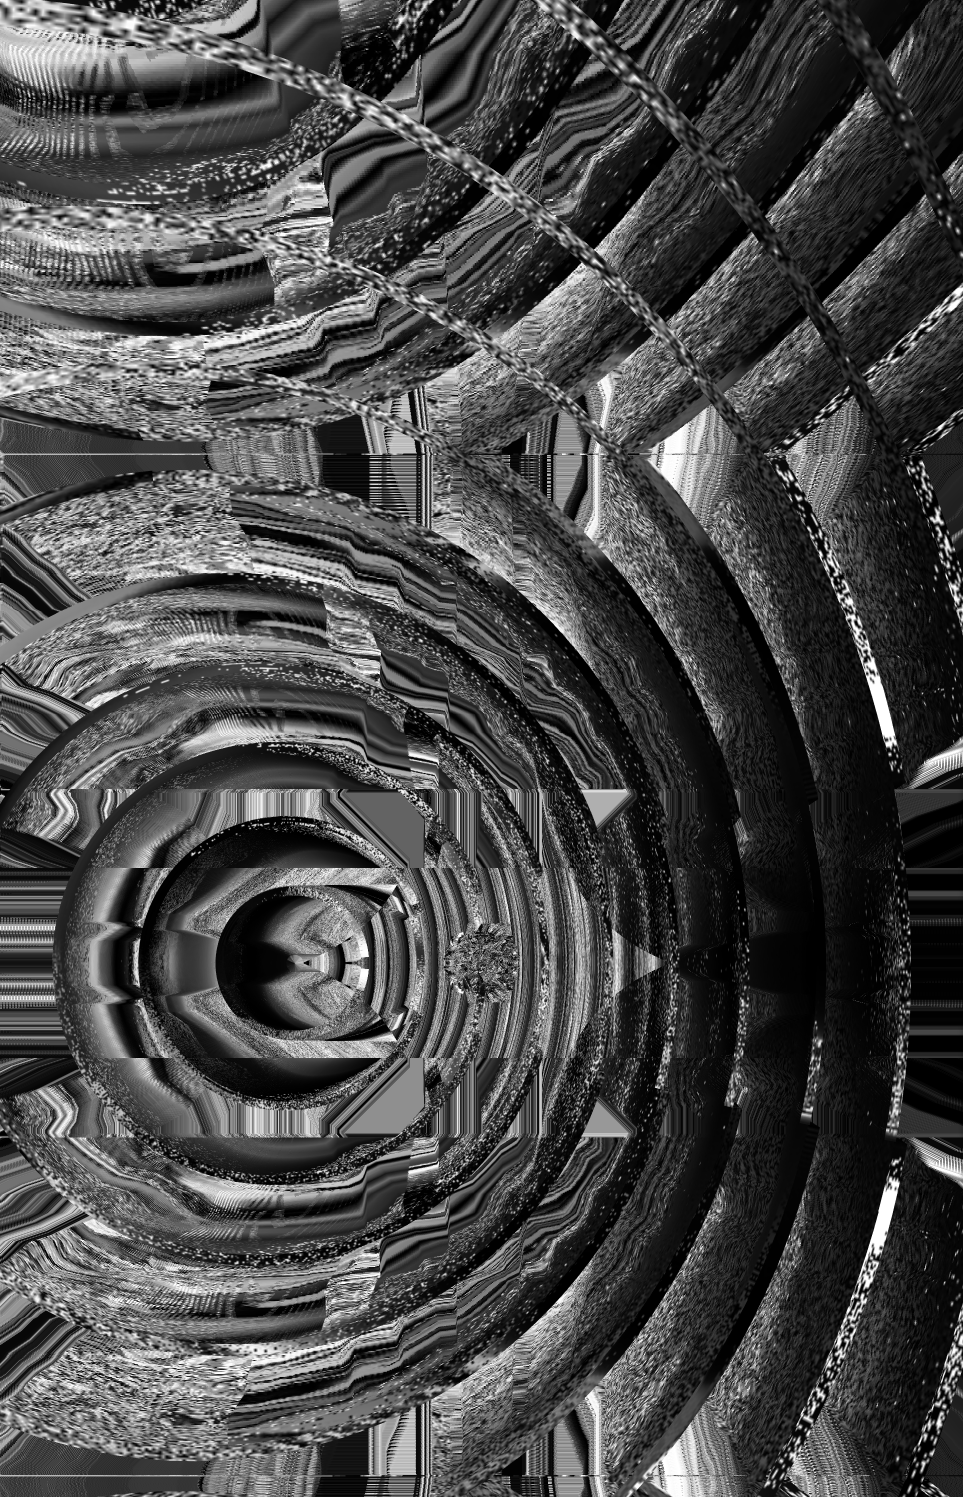
\includegraphics[width=\paperwidth,height=\paperheight]{../../img/portada.png}};
    
   
    \begin{center}
      
      \raggedleft 
                                                   
             {\bfseries\LARGE Universidad Nacional Autónoma de México \par}                                                                                                                
             \vspace{0.5cm}                                                                                                                                                                  
             {\scshape\Large Programa de Maestría y Doctorado en Música \par}
                  
             \vspace{0.5cm}                                                                                                                                                          
           
           {\scshape\large Facultad de Música \par}
           {\scshape\large Instituto de Ciencias Aplicadas y Tecnología \par}
           {\scshape\large Instituto de Investigaciones Antropológicas \par}

           \vfill
           \vspace{0.5cm}
        
                  
           {\scshape\Huge   Tres Estudios Abiertos \\

             % El siguiente subtitulo tiene que cambiar, ajustar a las preguntas de investigación
             
             % \Large Prácticas performáticas audiovisuales y experimentales, con lenguajes de programación\par}

             \Large Escrituras audiovisuales para el navegador\par}
            
             
                  %\vspace{1cm}
                  
        %      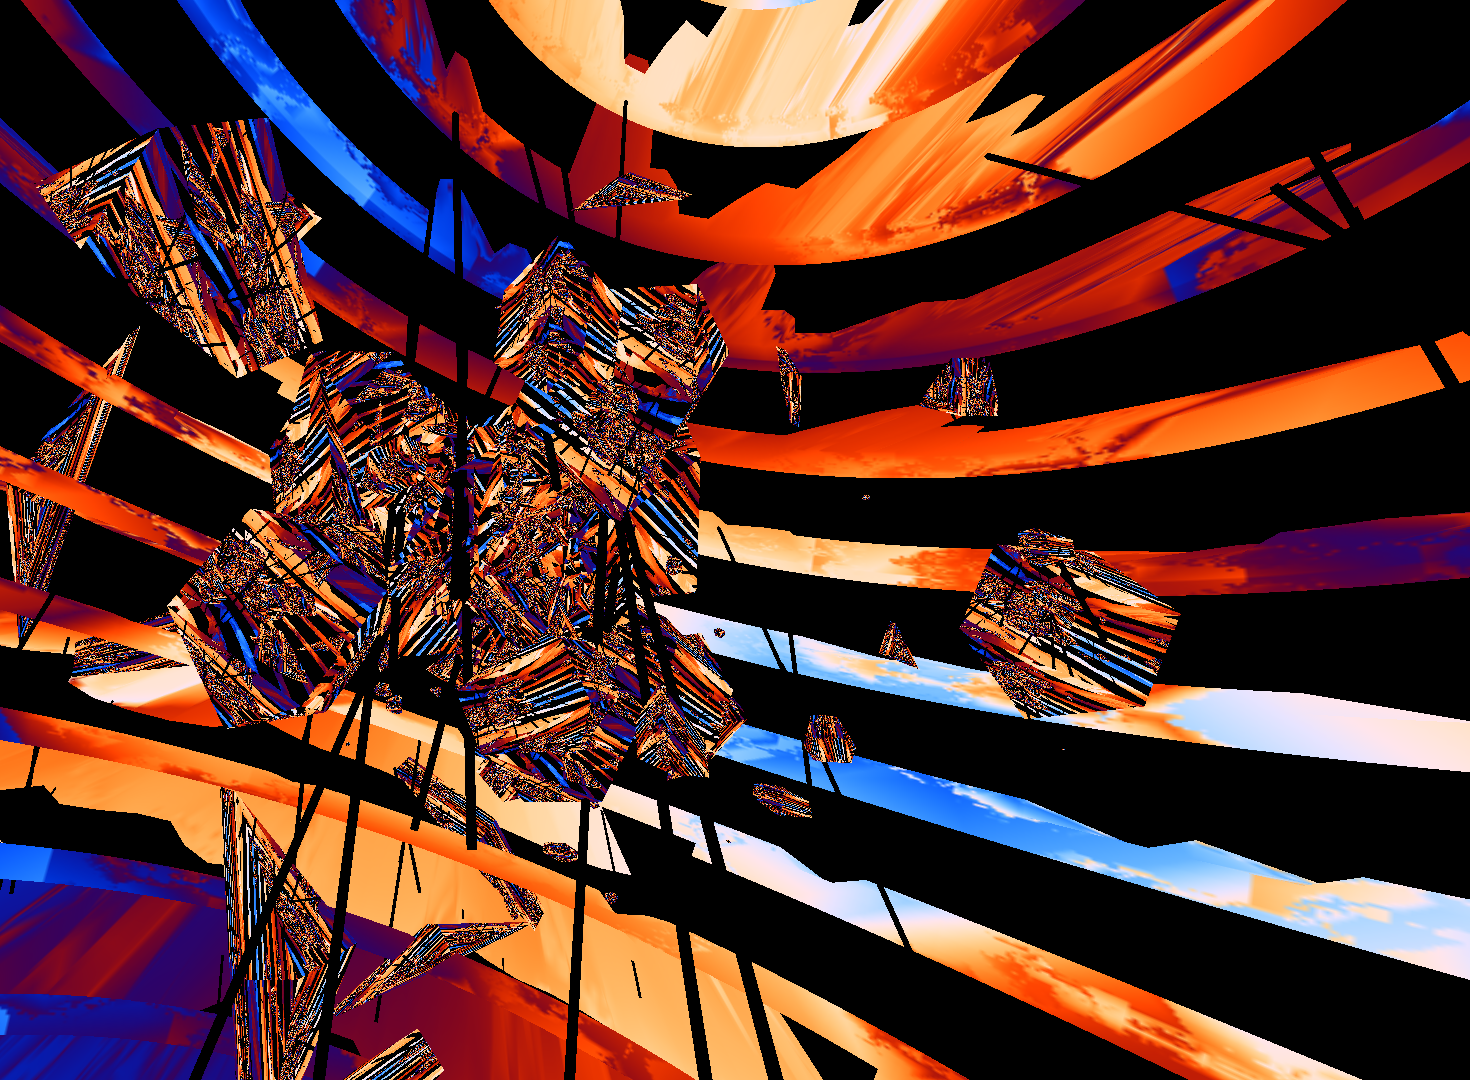
\includegraphics[width=0.5\textwidth]{../../img/error2.png}

           
           \vspace{0.5cm}
       
                     \vfill                                                                   
           {\scshape\large Que para optar por el grado de\\
             Doctor en Música\\
             (Tecnología Musical)\\\par}                                        
%{\itshape\Large Proyecto Fin de Carrera \par}                                                                                                                                
\vspace{0.5cm}                                                                                                                                                                        
%{\Large Autor: \par}
    {\scshape\large Presenta\\
      Emilio Ocelotl Reyes\\
      Tutor principal: Hugo Solís García\\
      Comité Tutor: Iracema e Andrade, Fernando Monreal\par}                                                                                                                                            
\vspace{0.5cm}                                                                                                                                                                  
    {\large \today \par}

    \end{center}                                                              

                                                                          
\end{titlepage}                                                                                                                                                               

\end{document}
